
\documentclass[12pt, a4paper]{report}

\usepackage{epsfig}
\usepackage{subfigure}
%\usepackage{amscd}
\usepackage{amssymb}
\usepackage{graphicx}
%\usepackage{amscd}
\usepackage{amssymb}
\usepackage{subfiles}
\usepackage{framed}
\usepackage{subfiles}
\usepackage{amsthm, amsmath}
\usepackage{amsbsy}
\usepackage{framed}
\usepackage[usenames]{color}
\usepackage{listings}
\lstset{% general command to set parameter(s)
basicstyle=\small, % print whole listing small
keywordstyle=\color{red}\itshape,
% underlined bold black keywords
commentstyle=\color{blue}, % white comments
stringstyle=\ttfamily, % typewriter type for strings
showstringspaces=false,
numbers=left, numberstyle=\tiny, stepnumber=1, numbersep=5pt, %
frame=shadowbox,
rulesepcolor=\color{black},
,columns=fullflexible
} %
%\usepackage[dvips]{graphicx}
\usepackage{natbib}
\bibliographystyle{chicago}
\usepackage{vmargin}
% left top textwidth textheight headheight
% headsep footheight footskip
\setmargins{1.0cm}{0.75cm}{18.5 cm}{22cm}{0.5cm}{0cm}{1cm}{1cm}
%\voffset=-2.5cm
%\oddsidemargin=1cm
%\textwidth = 520pt

\renewcommand{\baselinestretch}{1.5}
\pagenumbering{arabic}
\theoremstyle{plain}
\newtheorem{theorem}{Theorem}[section]
\newtheorem{corollary}[theorem]{Corollary}
\newtheorem{ill}[theorem]{Example}
\newtheorem{lemma}[theorem]{Lemma}
\newtheorem{proposition}[theorem]{Proposition}
\newtheorem{conjecture}[theorem]{Conjecture}
\newtheorem{axiom}{Axiom}
\theoremstyle{definition}
\newtheorem{definition}{Definition}[section]
\newtheorem{notation}{Notation}
\theoremstyle{remark}
\newtheorem{remark}{Remark}[section]
\newtheorem{example}{Example}[section]
\renewcommand{\thenotation}{}
\renewcommand{\thetable}{\thesection.\arabic{table}}
\renewcommand{\thefigure}{\thesection.\arabic{figure}}
\title{Research notes: linear mixed effects models}
\author{ } \date{ }


\begin{document}
\author{Kevin O'Brien}
\title{LME Models for Method Comparison Studies}
%\tableofcontents

\chapter{A Simplified LME Framework for Method Comparison}
\section{Agreement Criteria for Replicate Measurements}


Varying degrees of importances should be attached to each the three agreement criteria listed by \citet{Barnhart}. Between-item variance $d^2_i$ is fundamentally a measure of the variability of the item-wise means, as measured by method $i$, but it does contain limited information on the precision of that method. 

For conventional method comparison problems, both methods measures the same set of items using the same unit of measurement. Convergence to equality of between-item variance is inevitable as the number of items $n$ increases. Significantly different estimates for $d^2_1$ and $d^2_2$ should not be expected for any practical problem. 

Therefore a violation of third criterium (i.e. different between-item variances) criterium is contingent upon, and a  
possible consequence of, the violation of the other two agreement criteria. However, a violation of the third criterium will not occur in isolation. As noted elsewhere, the matter of inter-method bias can be easily accounted for, once detected. Both between-items and within-items variances must be calculated such that sources of variances are properly assigned, and to compute limits of agreement. However, testing the within-item criterium is the most informative analysis and therefore requires the most attention. 

\section{A Review of Criteria for Agreement in Roy's Framework}

\citet{ARoy2009} proposes a suite of hypothesis tests for assessing the agreement of two methods of measurement, when replicate measurements are obtained for each item, using an LME framework. For this framework, \citet{ARoy2009} recalls three criteria from \citet{Barnhart} for two methods to be considered in agreement (which are presented here in a different order);

\begin{enumerate}
\item There be no significant inter-method bias between the two methods, i.e. there is no persistent tendency for one method to give higher values than the other.
\item There is no difference in the within-subject variabilities, i.e. no significant difference in the random error among the replications taken by the same method on the same subject. 
\item There is no significant difference in the between-subject variabilities, the variances of the mean measurements for each case from both methods are not significantly different.
\end{enumerate} 
\citet{ARoy2009} demonstrates a LME model specification, and a series of tests that look at each of these agreement criteria individually. If two methods of measuement lack agreement, the specific reason or reasons for this lack of agreement can be identified. \citet{ARoy2009} further proposes examination of the the overall variability by considering the second and third criteria be examined jointly. Should both the second and third criteria be fulfilled, then the overall variabilities of both methods would be equal.

\citet{ARoy2009} provides an adjusted set of criteria, considering two methods to be in agreement if three conditions are met. Firstly that there is no significant bias, i.e. the difference between the two
mean readings is not ``statistically significant". Secondly there is
agreement between the two methods by testing their
repeatability coefficients. Finally, that there is a high overall correlation coefficient between methods for agreement to be present.


%\section{Critiquing the Relevance of Third Criterion}
Criteria 1 and 2, as listed above, are extensions of key statistical properties of accuracy and precision, which are discussed by \citet{Barnhart} in the context of method comparison, and can be considered as essential when comparing methods of measurement, with no further discussion required.

%\citet{Barnhart} describes the sources of disagreement as differing population means, different between-subject variances, different within-subject variances between two methods and poor correlation between measurements of two methods.

The third criteria concerns the equality of between-method variances, and is the basis of one of Roy's three tests. \citet{ARoy2009} remarks that between-subject variabilities are needed when the interest lies in the true or real difference between the two methods giving different measurements on the same subject, and are crucial when one is concerned about the true difference between the two methods \citep{ARoy2009}. Constructively the null hypothesis of this test calls for the equality of variances of the mean measurements 
for both sets of measurements. From a theoretical point of view, this criterion is a valid requirement for method agreement. 

However, one should consider how a violation of this criterion could occur. When items are measured on the same scale by both methods, the resulting measurements should be numerically near to each other on a consistent basis, even in the absence of agreement, even with a very small data set. 

\citet{ARoy2009} points out that sometimes there can be significant difference in between-subject variabilities of the two methods. The presence of proportional bias will give rise to a significant difference in between-subject variance. While this is correct, the proportional bias must be very drastic for it to cause a difference in between subject variabilities. If proportional bias is not present, there must be a catastrophic failure of one or both of the measurement methods, i.e. they are systematically unable to yield a pair of measurements for an item that are numerically close together.

If this was the case, this phenomenon would be immediately identifiable in the exploratory phase of the analysis, i.e. from a visual inspection of the scatterplot, and from fundamental summary statistics. A complicated model framework, such as an LME model, would not be required to determine this outcome. Furthermore, such is the complexity of LME models, that a solution may be intractable.

For comparing two methods of measurement, using different scales of measurement, (e.g. Celsium and Fahrenheit), a difference in between-subject variability is to be expected. However this scenario is outside of the scope of the typical method comparison study. 

As such, the test of this third criterion should not be conducted simultaneously with tests for the other two, as proposed by \citet{ARoy2009}. Instead violation of Criteria 3 should be determined early in the model building phase. No useful analysis can be carrried out if a violation exists. Violations of criteria 1 and 2 may exist in the context of two functioning measurement systems, as demonstrated in the examples provided by \citet{ARoy2009}.


\section{Towards A Simplified Model Framework}
\citet{BA99} recommended simultaneous estimation of repeatability and agreement
for replicate measurements. When no longer required to simultaneously test for a violation of the third criteria, we are afforded the opportunity to test the first two criteria with a LME model framework that is simpler than Roy's model. A violation of the first criterion can be detected by inspection of the estimate for the fixed effects. A violation of the second criterion can be detected by an inspection of the residuals.

An advantage of using a simplified LME framework is that it affords the opportunity to test Criteria 1 and 2 for more than two methods of measurement simultaneously. Both \citet{BA99} and \citet{ARoy2009} use as an example the simultaneous measurements of systolic blood pressure
were made by each of the two experienced observers (denoted by J and R) using a sphygmomanometer, and by a semi-automatic blood pressure monitor (denotedby S). Three sets (p = 3) of readings were made in quick succession on 85 subjects. 

The following approach shows that it can be quickly determined which pair of methods are in agreement.

\begin{description}
\item[Step 1] A LME model is fitted to the entire data set. A fixed effect is used to represent the measurement methods. The random error is collected in a random effect. For the sake of simplicity, one of the measurement methods can be chosen as the base case.

\item[Step 2] A test of criterion 1 can be implemented by an examination of the fixed effects. While the creators of the LME4 R package advised against the use of p-values, a set of confidence intervals can be determined.

\item[Step 3] A test of criterion 2 can be implemented by an examination of the residuals. An omnibus test for all $p$ methods together can be implemented as a Bartlett Test of homogeneity of variances. Pairwise comparison may be implemented using the standard $F-$test for equality of variance. Both tests are facilitated by most statistical software packages.
\end{description}

Further insights can be made using influence diagnostic procedures, such as Cook's Distance and DFBETAs, and will be reverted to.


The LME model proposed by \citet{ARoy2009} should be retained in the overall method comparison framework, as it is still strongly preferred for computing limits of agreement and the repeatability coefficient.
\citet{ARoy2009} states the importance of reporting repeatability when assessing measurement, because it measures the purest
random error that is not influenced by any other factors \citep{Barnhart}.
\citet{ARoy2009} advises against the use any kind of correlation coefficient for assessing agreement for data with replications, even though that framework allows for the computation of the overall correlation coefficient.


%Strong positive correlation between measurements set, to some degree, should be expected between both sets of measurements.

\newpage

\begin{verbatim}
## Step 1. Load R packages
library(dplyr);  library(magrittr);  library(broom)
library(lme4)
library(GGally)

## Step 2. Get the Blood Pressure Data
source("https://raw.githubusercontent.com/DragonflyStats/MCS-code/master/blooddata.R")

## Step 3. Fit the Simplified LME Model
MCSModel <- lmer(BP ~ method + (1|subject),data=blood)

## Step 4. Test the inter-method bias criterion, i.e. criterion 1.
summary(MCSModel)
ggcoef(MCSModel)  # visual analogue

## Step 5. Augment the Blood data set with additional estimates
blood <- augment(MCSModel,blood)

## Step 6. Compare Estimate for Residal Variances
blood %>% group_by(method) %>% summarize(Sigma.sq.W = var(.resid)) 

## Step 7. Omnibus Test for Equality of Variances
bartlett.test(.resid~method,data=blood)

## Step 8. Pairwise Test for Equality of Variances
blood.js <- blood %>% filter(method %in% c("J","S"))
var.test(.resid~method,data=blood.js)

\end{verbatim}
\section{Using DFBETAs from LME Models to Assess Agreement}

DFBETA and DFFITS are well known measures of influence. Emphasis shall be placed on DFBETA, but a brief discussion of DFFITS is merited as it potentially provides for useful techniques in method comparison. \citet{schabenberger} provides a mathematical desciption of both.


DFBETAS is a standardized measure of the absolute difference between the estimate with a particular
case included and the estimate without that particular case,, thus measuring the impact each observation has on a particular predictor \citep{belsley2005}. For LME models, the DFBETA is a measure that standardizes the absolute difference in parameter estimates between an LME model based on a full set of data, and a model from reduced data.

In general, large values of DFBETAS indicate observations that are influential in estimating a given parameter. There is no agreement as to the critical threshold for DFBETAs. \citet{belsley2005} recommend 2 as a general cutoff value to indicate influential observations and as a size-adjusted cutoff.  The cut-off value for DFBETAs is $\frac{2}{\sqrt{n}}$, where $n$ is the number of observations. 



\subsubsection{Using DFBETAs for Method Comparison}
For LME models, a value for DFBETAS is calculated for each of the $p$ fixed effects, and for each of the $n$ item. When the LME model is specified without an intercept term, as in Roy's Model, there is a set of DFBETAs corresponding to each measurement method, hence an $n \times p$ matrix.
% Correctly there will be $p+1$ DFBETAs (the intercept, $\beta_0$, and one $\beta$ for each covariate)

The LME approach proposed by \citet{ARoy2009} is constrained by computational tractability. Consequently a simpler LME formulation is used, one similar to that of \citet{BXC2008}. However one constraint that can be dispensed with is the restriction to two methods of measurement: we can now use any number of methods. The benefit of using this model is that metrics such as Cook's Distance and DFBETAs can be computed also.

For a method comparison study, DFBETAs can be used as a proxy measurement, allowing simple techniques to be used for assessing agreement. Suppose an LME model was formulated to model agreement for two or more methods of measurement, specifically with replicate measurements.

Hence, commonly used bivariate analyses constructed to compare each pair of methods, based on their respective sets of DFBETAs. Furthermore 95\% confidence ellipse can be constructed around these scatterplots. If the methods are to be agreement, the DFBETAs for each case would be the same for both methods. As such, agreement between any two methods can be visually inspected from a scatterplot of the DFBetas. 


%%
%%Furthermore, these measures form the basis of the analysis, rather than the estimates derived from the model. In the context of method comparison, these variables are the methods of measurement. Agreement will considered in the context of inter-method bias and the within-item variance ratio. Between-item variance ratio is not considered for this analysis.

Following the idea proposed by \citet{BA86}, an identity plot to visually inspect this relationship between sets of DFBETAs. Modern statistical software usually allows for the creation of co-plots, so a grid of identity plots may be easily rendered for comparing each pair of methods.

If the lack of agreement is caused, in part or in full, by differing within-item variances, there would be differing DFBETAs for each pair of methods. If the points align along the line of equality, then both methods can be said to be in agreement for within item variance. However DFBETAs are not useful for determining inter-method bias. 

If there is good agreement between methods, or if lack of agreement is caused by inter-method bias only, the DFBETA values will be almost identical for each subject. Therefore this plot should be used in conjunction with a Bland-Altman plot. If lack of agreement is indicated, a comprehensive analysis using Roy's framework can be used to formally test for various causes of lack of agreement \citep{ARoy2009}.



For an LME model fitted to the Systolic Blood Pressure data, the results tabulated below can be produced.  Cases can be ranked by the Cook's Distance, with the top 6 being presented below). The remaining columns are the DFBeta for each of the fixed effects, for each of the 85 subject.
\begin{center}
	\begin{tabular}{|c|c|c|c|c|} \hline
		Subject &    Cook's D  &    Method J  &   Method R  & Method S \\ \hline \hline
		78 & 0.6155 & -0.0293 & -0.0338 & 0.2954  \\ \hline
		80 & 0.4159 & -0.0630 & -0.0651 & 0.2123  \\ \hline
		68 & 0.2253 & -0.0533 & -0.0506 & 0.1555  \\ \hline
		72 & 0.0934  & 0.0238  & 0.0241 & 0.1617  \\ \hline
		48 & 0.0870  & 0.0214  & 0.0314 & 0.1581  \\ \hline
		30 & 0.0711  & 0.2692  & 0.2621 & 0.1581  \\ \hline
	\end{tabular}
\end{center}
For DFBETA identity plots are presented in Figure~\ref{fig:04-DFbetaplots}. This set of plots indicate agreement between methods J and R in terms of within-item variance, while severe lack of agreement exists between these methods and the third method S, as is the conclusion of \citet{ARoy2009}.
\begin{figure}[h!]
	\centering
	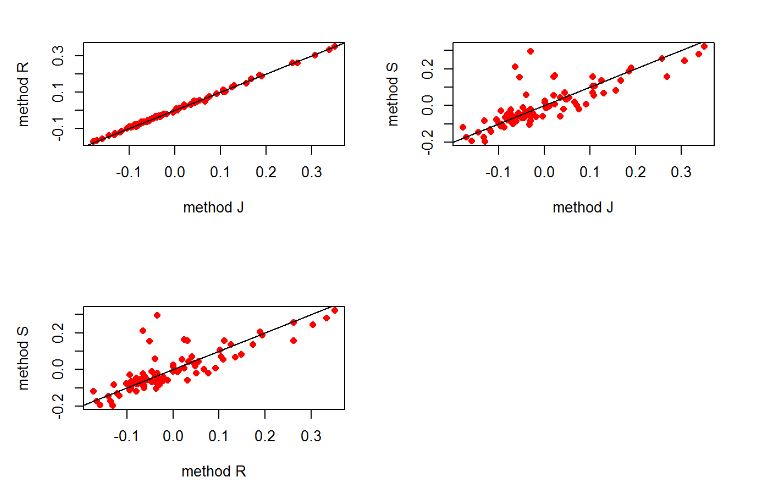
\includegraphics[width=1.1\linewidth]{images/04-DFbetaplots}
	% \caption{}
	\label{fig:04-DFbetaplots}
\end{figure}



%Other analyses may be used to complement these plots. The Pearson Correlation coefficient of the DFBETAs can be used in conjection with this analysis. A high correlation confirms good agreement, thouhg no threshold value for agreement is suggested.

The Bonferroni Outlier Test and Cook's Distance values can be used to identify unusual cases, when the relationship between sets of DFBETA is modelled as a (classical) linear model. In this model, the covariates should be homoskedastic. A test for non-constant variance may be used to verify this. 


As an alternative to scatterplots, a mean difference plot could be used to assess agreement of with-item variance. This mean-difference plot differs from the Bland-Altman plot in that the plot is denominated in terms of DFBETA values, and not in measurement units. Here two of the three pairs of methods are compared on the same plot, red points indicate the J-R comparison while blue points are for the J-S comparison.

\begin{figure}[h!
	]
	\centering
	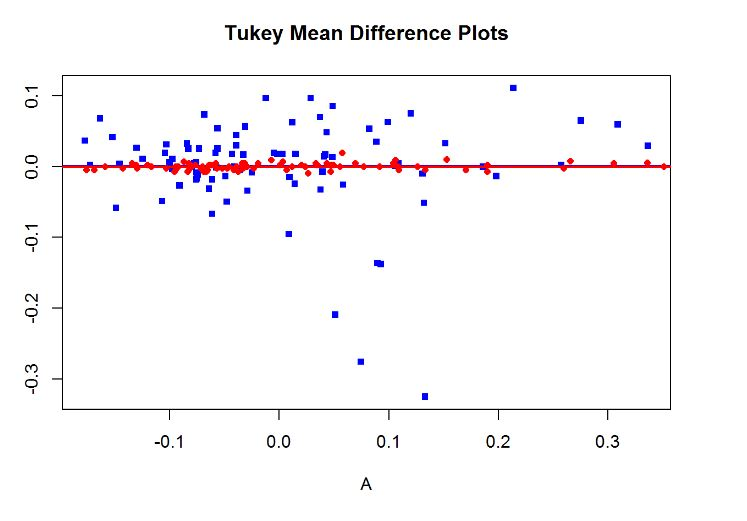
\includegraphics[width=0.7\linewidth]{images/04-TMDplot}
	
\end{figure}

\bibliographystyle{chicago}
\bibliography{2017bib}
\end{document}
